% Hlavicka pro protokoly z fyzikalniho praktika.
% Verze pro: LaTeX
% Verze hlavicky: 22. 2. 2007
% Autor: Ustav fyziky kondenzovanych latek
% Ke stazeni: www.physics.muni.cz/ufkl/Vyuka/
% Licence: volne k pouziti, nejlepe k vcasnemu odevzdani protokolu z Vaseho mereni.


\documentclass[czech,11pt,a4paper]{article}
\usepackage[T1]{fontenc}
\usepackage{graphicx}
\usepackage{mathtools}
\usepackage{amssymb}
\usepackage{amsthm}
\usepackage{thmtools}
\usepackage{xcolor}
\usepackage{nameref}
\usepackage{babel}
\usepackage{hyperref}
\usepackage{multicol}
\usepackage[export]{adjustbox}
\usepackage{subcaption}
\usepackage{caption}
\usepackage{multirow}
\usepackage{float}
\usepackage{placeins}




%%% Nemente:
\usepackage[margin=2cm]{geometry}
\newtoks\jmenopraktika \newtoks\jmeno \newtoks\datum
\newtoks\obor \newtoks\skupina \newtoks\rocnik \newtoks\semestr
\newtoks\cisloulohy \newtoks\jmenoulohy
\newtoks\tlak \newtoks\teplota \newtoks\vlhkost
%%% Nemente - konec.


%%%%%%%%%%% Doplnte pozadovane polozky:

\jmenopraktika={Fyzikální praktikum 1}  % nahradte jmenem vaseho predmetu
\jmeno={Teodor Duraković}            % nahradte jmenem mericiho
\datum={15.~května 2024}        % nahradte datem mereni ulohy
\obor={F}                     % nahradte zkratkou vami studovaneho oboru
\skupina={St 8:00}            % nahradte dobou vyuky vasi seminarni skupiny
\rocnik={I}                  % nahradte rocnikem, ve kterem studujete
\semestr={II}                 % nahradte semestrem, ve kterem studujete

\cisloulohy={4}               % nahradte cislem merene ulohy
\jmenoulohy={Měření gravitační konstanty a tíhového zrychlení} % nahradte jmenem merene ulohy

\tlak={98 \,\rm 512}                   % nahradte tlakem pri mereni (v hPa)
\teplota={24.0}               % nahradte teplotou pri mereni (ve stupnich Celsia)
\vlhkost={39.7}               % nahradte vlhkosti vzduchu pri mereni (v %)

%%%%%%%%%%% Konec pozadovanych polozek.


%%%%%%%%%%% Uzitecne balicky:

%%%%%% Zamezeni parchantu:
\widowpenalty 10000 \clubpenalty 10000 \displaywidowpenalty 10000
%%%%%% Parametry pro moznost vsazeni vetsiho poctu obrazku na stranku
\setcounter{topnumber}{3}	  % max. pocet floatu nahore (specifikace t)
\setcounter{bottomnumber}{3}	  % max. pocet floatu dole (specifikace b)
\setcounter{totalnumber}{6}	  % max. pocet floatu na strance celkem
\renewcommand\topfraction{0.9}	  % max podil stranky pro floaty nahore
\renewcommand\bottomfraction{0.9} % max podil stranky pro floaty dole
\renewcommand\textfraction{0.1}	  % min podil stranky, ktery musi obsahovat text
\intextsep=8mm \textfloatsep=8mm  %\intextsep pro ulozeni [h] floatu a \textfloatsep pro [b] or [t]

% Tecky za cisly sekci:
\renewcommand{\thesection}{\arabic{section}.}
\renewcommand{\thesubsection}{\thesection\arabic{subsection}.}
\renewcommand{\thesubsubsection}{\thesubsection\arabic{subsubsection}.}
% Jednopismenna mezera mezi cislem a nazvem kapitoly:
\makeatletter \def\@seccntformat#1{\csname the#1\endcsname\hspace{1ex}} \makeatother


%%%%%%%%%%%%%%%%%%%%%%%%%%%%%%%%%%%%%%%%%%%%%%%%%%%%%%%%%%%%%%%%%%%%%%%%%%%%%%%
%%%%%%%%%%%%%%%%%%%%%%%%%%%%%%%%%%%%%%%%%%%%%%%%%%%%%%%%%%%%%%%%%%%%%%%%%%%%%%%
% Zacatek dokumentu
%%%%%%%%%%%%%%%%%%%%%%%%%%%%%%%%%%%%%%%%%%%%%%%%%%%%%%%%%%%%%%%%%%%%%%%%%%%%%%%
%%%%%%%%%%%%%%%%%%%%%%%%%%%%%%%%%%%%%%%%%%%%%%%%%%%%%%%%%%%%%%%%%%%%%%%%%%%%%%%

\begin{document}
	
	%%%%%%%%%%%%%%%%%%%%%%%%%%%%%%%%%%%%%%%%%%%%%%%%%%%%%%%%%%%%%%%%%%%%%%%%%%%%%%%
	% Nemente:
	%%%%%%%%%%%%%%%%%%%%%%%%%%%%%%%%%%%%%%%%%%%%%%%%%%%%%%%%%%%%%%%%%%%%%%%%%%%%%%%
	\thispagestyle{empty}
	
	{
		\begin{center}
			\sf 
			{\Large Ústav fyzikální elektroniky Přírodovědecké fakulty Masarykovy univerzity} \\
			\bigskip
			{\huge \bfseries FYZIKÁLNÍ PRAKTIKUM} \\
			\bigskip
			{\Large \the\jmenopraktika}
		\end{center}
		
		\bigskip
		
		\sf
		\noindent
		\setlength{\arrayrulewidth}{1pt}
		\begin{tabular*}{\textwidth}{@{\extracolsep{\fill}} l l}
			\large {\bfseries Zpracoval:}  \the\jmeno & \large  {\bfseries Naměřeno:} \the\datum\\[2mm]
			\large  {\bfseries Obor:} \the\obor  \hspace{40mm}  {\bfseries Skupina:} \the\skupina %
			%{\bfseries Ročník:} \the\rocnik \hspace{5mm} {\bfseries Semestr:} \the\semestr  
			&\large {\bfseries Testováno:}\\
			\\
			\hline
		\end{tabular*}
	}
	
	\bigskip
	
	{
		\sf
		\noindent \begin{tabular}{p{3cm} p{0.6\textwidth}}
			\Large  Úloha č. {\bfseries \the\cisloulohy:} \par
			\smallskip
			$T=\the\teplota$~$^\circ$C \par
			$p=\the\tlak$~Pa \par
			$\varphi=\the\vlhkost$~\%
			&\Large \bfseries \the\jmenoulohy  \\[2mm]
		\end{tabular}
	}
	
	\vskip1cm
	
	%%%%%%%%%%%%%%%%%%%%%%%%%%%%%%%%%%%%%%%%%%%%%%%%%%%%%%%%%%%%%%%%%%%%%%%%%%%%%%%
	% konec Nemente.
	%%%%%%%%%%%%%%%%%%%%%%%%%%%%%%%%%%%%%%%%%%%%%%%%%%%%%%%%%%%%%%%%%%%%%%%%%%%%%%%
	
	%%%%%%%%%%%%%%%%%%%%%%%%%%%%%%%%%%%%%%%%%%%%%%%%%%%%%%%%%%%%%%%%%%%%%%%%%%%%%%%
	%%%%%%%%%%%%%%%%%%%%%%%%%%%%%%%%%%%%%%%%%%%%%%%%%%%%%%%%%%%%%%%%%%%%%%%%%%%%%%%
	% Zacatek textu vlastniho protokolu
	%%%%%%%%%%%%%%%%%%%%%%%%%%%%%%%%%%%%%%%%%%%%%%%%%%%%%%%%%%%%%%%%%%%%%%%%%%%%%%%
	%%%%%%%%%%%%%%%%%%%%%%%%%%%%%%%%%%%%%%%%%%%%%%%%%%%%%%%%%%%%%%%%%%%%%%%%%%%%%%%
	
	\section{Úvod}
	Tíhové zrychlení a gravitační konstanta jsou vlastnosti vycházející z jedné ze čtyř základních interakcí. Pro lidstvo je přesné změření tíhového zrychlení i gravitační konstanty klíčové pro mnoho kalkulací, ať již se jedná o meziplanetární síly a další astronomické výpočty, nebo o kalkulaci rychlosti padání ze schodů. Z mnoha způsobů měření těchto hodnot (s konstantami bychom si je plést neměli, jelikož je tíhové zrychlení hodnota závislá mj. na geografické poloze) tíhové zrychlení změříme prostřednictvím reversního kyvadla a~gravitační konstantu pomocí Cavendishových vah.
	
	
	
	\section{Zadání}
	\noindent1. Změřte tíhové zrychlení reverzním kyvadlem. Proměřte závislost T1(y) a T2(y) aspoň pro pět
	poloh závaží, sestrojte v programu QtiPlot graf a najděte polohu y0. V jejím okolí změřte periodu
	kmitů podrobněji tak, abyste upřesnili průsečík křivek T1(y) a T2(y). Změřte redukovanou délku
	kyvadla a~stanovte hodnotu tíhového zrychlení včetně nejistoty. Porovnejte výsledek s místní
	hodnotou.\\
	
	\noindent2. Změřte gravitační konstantu Cavendishovými torzními vahami. Zapněte laser pro monitoring
	zrcátka vah a na počítači spusťte záznam pohybu oscilátoru. Po cca 15 minutách zkuste měření
	na zkoušku vyhodnotit. 
	
	
	\section{Postup, metody měření}
	\subsection{Tíhové zrychlení}
	Při použití reverzního kyvadla využíváme skutečnosti, že při rovnosti period kmitů vzhledem k oběma osám můžeme vztah periody na redukované délce (vzdálenosti os) a tíhovém zrychlení můžeme zapsat jako:
	\begin{equation}
		T = 2 \pi \sqrt{\frac l g}
	\end{equation}
	Ke změření tíhového zrychlení nám tedy stačí sestrojit reverzní kyvadlo, které tuto vlastnost bude splňovat. Toho dosáhneme posuvným závážím na jednom konci kyvadla, jehož vzdálenost od konce upravíme tak, aby se periody rovnaly. 
	
	Nejdříve je tedy potřeba získat hodnotu redukované délky:
	\begin{equation}
		l = (0.99 \pm 3.10^{-4} )\,\rm m
	\end{equation}
	
	Dále budeme závaží posouvat a periody měřit pro kyvy přes dolní i horní uchycení. Získáváme:
	
	\begin{center}
			\begin{tabular}{c|c|c}
		d [cm] & Horní perioda [s] & Spodní perioda [s] \\ \hline
		2      & 1.978   & 1.921    \\ \hline
		3      & 1.987   & 1.954   \\ \hline
		4      & 1.995   & 1.990    \\ \hline
		5      & 2.003   & 2.025    \\
	\end{tabular}\\
	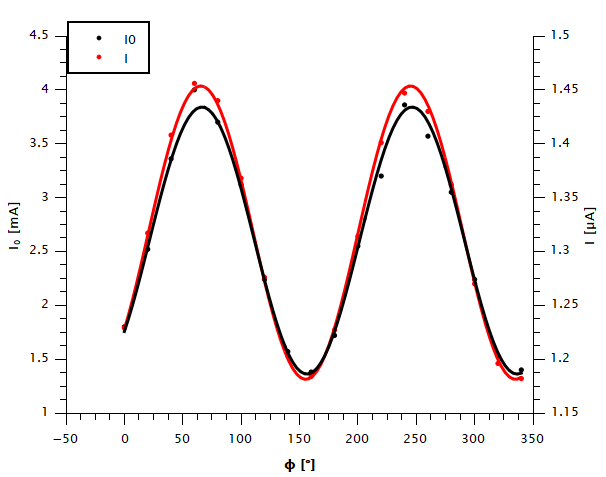
\includegraphics[width=0.75\linewidth]{zavislost}

	\end{center}
	Již z výše uvedené tabulky lze vidět, že se periody budou rovnat při umístění závaží mezi čtyřmi až pěti centimetry (využíváme měřítka na samotném kyvadle). Získaná data využijeme k tvorbě lineárních fitů a nalezneme průsečík obou přímek. Získáváme hodnotu:
	
	\begin{equation}
		d = (4.18 \pm 0.13) \,\rm cm
	\end{equation}
	Vidíme, že odchylka při odvození správné délky prostřednictvím fitu není nezanedbatelná a že bychom se k hodnotě vzdálenosti pro stejnou periodu pravděpodobně mohli dostat jednodušeji realizací menších změn nad hranicí čtyř centimetrů. Využijeme však získané hodnoty a zhodnotíme vzájemnou odchylku period. Uvedenou polohu závaží se pokusíme realizovat posuvným měřítkem a měření periody pro oba způsoby zavěšení provedeme devadesátkrát, abychom získali hodnoty statistických odchylek a přesnou standardní nejistotu:
	
	\begin{center}
		\begin{tabular}{c|c|c}
			d [cm] & Horní perioda [s] & Spodní perioda [s] \\ \hline
			4.18      & 1.99614 $\pm 1.7.10^{-5}$  & 1.99616 $\pm 1.3.10^{-5}$    \\ 
		\end{tabular}\\
	\end{center}
		
		Vidíme, že se periody odchylují až v řádech \textbf{statisícin}, i přes neperfektní postup (odchylka odhadnuté periody poměrně narušovala směrodatnost získané hodnoty) jsme tedy dostali velice přesný výsledek.
		
		Jelikož hledáme hodnoty period, při kterých se budou rovnat, a zároveň víme, že funkce periody na vzdálenosti rostou se vzdáleností lineárně, můžeme z hodnot periody pro horní a spodní zavěšení spočítat aritmetický průměr, jelikož jiný způsob přiblížení ke správnému výsledku není v našich silách - pokud bychom periodu chtěli upravit posunutím závaží, posouvali bychom jej v řádech mikrometrů, což by se nám nejspíše nepodařilo.
		Statistickým přiblížením tedy získáme hodnotu:
		\begin{equation}
			T = 1.99615 \pm 1.10^{-5}\,\rm s
		\end{equation}
		Při úpravě formule (1) získáme formuli pro výpočet tíhového zrychlení:
		\begin{equation}
			g = l \left(\frac{2\pi }{T}\right)^2
		\end{equation}
		Pro tíhové zrychlení získáváme hodnotu:
		\begin{equation}
			g = 9.809 \pm 0.003 \,\rm m.s^{-2}
		\end{equation}
		Spočítáme-li tíhové zrychlení za použití relace \\ $ g = [9,780 356(1 + 0,005 288 5 \sin^2 \phi - 0,000 005 9 \sin^2
		2 \phi) - 0,000 003 086 H ]$ uvedené v návodu praktika$^{[1]}$, kde $\phi $ je zeměpisná šířka a $H$ nadmořská výška, získáme hodnotu  $g = 9.8092 \,\rm m.s^{-2}$, vidíme, že se od této hodnoty odchylujeme pouze o cca. šest desetitisícin. Získali jsme tedy \textbf{velice přesný výsledek.}
		\subsection{Gravitační konstanta}
		Cavendishovy torzní váhy prostřednictvím precizní konstrukce eliminují gravitační vliv Země na měření působení gravitačních sil mezi dvěma hmotnými koulemi a dvojicí malých kuliček, přičemž tyto kuličky jsou zavěšeny na torzním vlákně, ke kterému je připevněno i malé zrcadlo, které můžeme využít pro odraz laserového paprsku na vzdálený objekt, čímž můžeme měřit velmi malé výchylky v torzi. 
		Experiment provedeme tak, že koule ke kuličkám (čince) přiblížíme z jedné strany, počkáme, až se činka ustálí a následně koule k čince přiblížíme z druhé strany a znovu počkáme pro realizaci "ustáleného" stavu. Z rozdílu výchylek dokážeme odvodit gravitační konstantu.
		
		\subsubsection{Analýza dat}
\begin{center}
			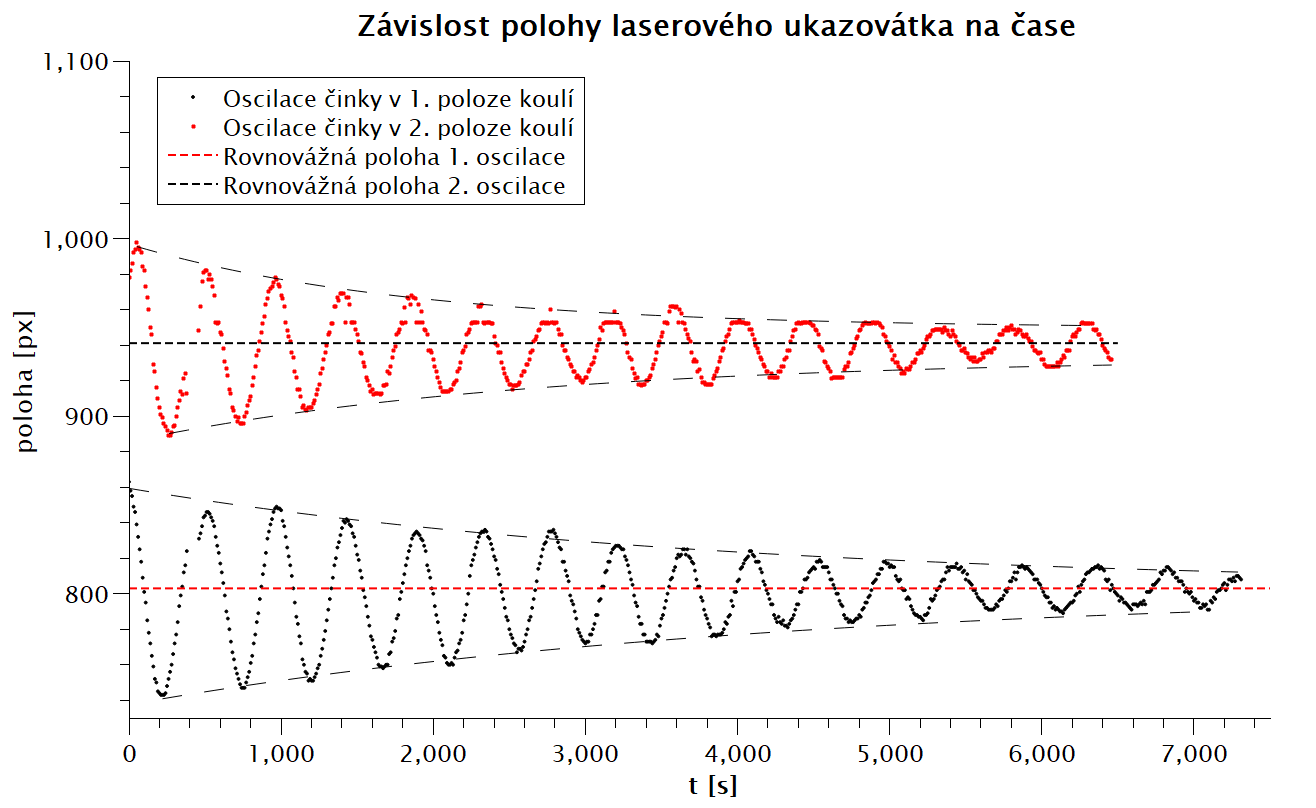
\includegraphics[width=0.89\linewidth]{Oscilace}
\end{center}
	Po přiblížení koulí k čince vidíme, že se činka gravitačním působením přesouvá a začíná oscilovat kolem jisté rovnovážné polohy. Pozorujeme exponenciálně tlumenou harmonickou oscilaci, čehož využíváme pro určení rovnovážné polohy. Izolujeme lokální maxima a minima obou setů a získané body proložíme funkcí $y_0 + A.e^{-\frac{x}{t}}$, právě $y_0$ by se pro páry maxim a minim měla rovnat a určovat hodnotu rovnovážné polohy. Reálné hodnoty se však mírně odchylují, proto z nich vytvoříme aritmetický průměr a tuto hodnotu uvažujeme jako polohu v rovnovážném stavu. Získáváme:
	
		\begin{align*}
		d_{1a} &= (804 \pm 5) \, \text{px}\\
		d_{1b} &= (802 \pm 11)\, \text{px} \\ 
		d_{2a} &= (933 \pm 4) \, \text{px} \\
		d_{2b} &= (949 \pm 2) \, \text{px} \\ \\
		D_1 &= (803 \pm 6) \, \text{px}\\
		D_2 &= (941.1 \pm 2) \, \text{px}\\ \\
		\Delta D &= (138 \pm 6) \,\text{px}
	\end{align*}
	Z analýzy pravítka o délce 500mm na snímcích zároveň získáme jeho rozměř v pixelech:
	\begin{equation*}
		l = (471.93 \pm 0.18) \,\rm px
	\end{equation*}
	Dále porovnáme rozměr pravítka v pixelech s rozměrem skutečným, abychom získali převodní vztah pro reálnou vzdálenost rovnovážných poloh
	\begin{equation*}
		k = \frac{500}{l} = 1.0595 \pm 0.0004
	\end{equation*}
	Pro skutečnou vzdálenost rovnovážných poloh platí
	\begin{equation*}
		\delta = \Delta D \cdot k = 146 \pm 6 \,\rm mm
	\end{equation*}
	
		Jelikož známe vzdálenost aparatury od zdi $(x = 5280 \pm 3 \,\rm mm)$, na kterou je obraz promítán, úhel mezi polohami získáme následovně:
		\begin{align*}
			\varphi = \arctan \frac{\delta}{x} = \arctan \frac{146}{5280} &= 0.0277 \pm 0.0012 \,\text{rad} \\ 
			&= 1.59 \pm 0.07^\circ
		\end{align*}
		
		Po získání výchylky spočítáme moment setrvačnosti kuliček vzhledem k ose závěsu:
		\begin{equation}
			J = 2m (\frac 2 5 \rho ^2 + d^2) = 1.936\cdot10^{-4} \pm 1\cdot10^{-6}\,\rm kg.m^2
		\end{equation}
		kde $m$ je hmotnost kuliček, $\rho$ jejich poloměr a $d$ vzdálenost mezi středem kuličky a osou závěsu.
		
		Pro kalkulaci direkčního momentu z dat získáme hodnotu periody:
		\begin{equation*}
			T = 500 \pm 13 \,\rm s
		\end{equation*}
		\begin{equation}
			D = \left(\frac{2 \pi}{T}\right)^2 J = 3.84 \cdot 10^{-8} \pm 0.07 \cdot 10^{-8} \,\rm \frac{kg.m^2}{s}
		\end{equation}
		
		Velikost momentu gravitační síly získáme formulí
		\begin{equation}
			M_{grav} = \varphi D 
		\end{equation}
		Musíme však uvažovat s čtvrtinovou hodnotou výchylky, jelikož chceme výchylku situace bez \\koulí/s koulemi (první snížení hodnoty dvakrát) a odrazem od zrcadla získáváme dvakrát větší výchylku, než je výchylka samotné činky (druhe zmenšení výchylky dvakrát). Získáváme:
		\begin{equation}
			M_{grav} = \frac \varphi 4 D = 2.66 \cdot 10^{-10} \pm 0.13 \cdot 10^{-10} \,\rm N m
		\end{equation}
		
		K získání hodnoty gravitační konstanty využijeme vzorce
		\begin{equation}
			G = \frac{M_{grav}}{2 (Mm)d(\frac{1}{r^2}-\frac{r}{(4d^2+r^2)^\frac{3}{2}})}
		\end{equation}
	 kde r je vzdálenost středu vetší koule od středu bližší malé koule a d je vzdálenost středu malé koule od osy závěsu. Po velmi vyčerpávajícím procesu se dostáváme k hodnotě:
	 
	 \begin{equation}
	 	G = 8.6 \cdot 10^{-11} \pm 0.6 \cdot 10^{-11} \,\rm \frac{m^3}{kg.s^2}
	 \end{equation}
	 která se bohužel od skutečné hodnoty značně odchyluje.
	
	
	
		
	

  
	
	\section{Závěr}
	Hodnotu tíhového zrychlení se nám podařilo získat překvapivě přesně, podstatnou roli zde mimo profesionality hrálo i štěstí, jelikož se nám k rovnosti obou period podařilo přiblížit hned při prvním finálním zachycení závaží. Jednoduchost tohoto úkolu naštěstí nenechala velký prostor pro chyby.
	Gravitační konstanta, respektive její měření, nám dalo hlavně zkušenost, že delší doba provádění experimentu nemusí nutně znamenat přesnější výsledek. Dostali jsme se do nádherně kontrastní situace, kdy první, jednodušší úkol přinesl nádherné závěry, zatímco výsledky druhé úlohy fakticky pro další kalkulace nejsou použitelné. Samozřejmě zde enormní roli hraje skutečnost, že imperfektní aparaturou a postupem měříme extrémně malou hodnotu, u které se jakákoliv, byť sebemenší odchylka projeví naprosto viditelně. Retrospektivně je jedním z hlavních nedostatků vizuální analýza, jelikož je rozlišení kamery pro tento účel poměrně nízké, zároveň věříme, že by zvýšení vzorkovací frekvence (resp. pořizování fotografií záznamu) mohlo měření značně upřesnit. Při opravě těchto nedostatků bychom byli schopni získat mnohem přesnější hodnoty periody i rovnovážné polohy, jelikož by došlo k eliminaci různých skoků ("nespojitostí") v křivkách výchylky.
	% Nakonec nezapomeňte projet text programem vlna nebo vlnka, např.
	% 	vlna -m -l -n mojeuloha.tex
	% nebo zkontrolovat a opravit jednopísmenné předložky na koncích řádků ručně.
	\section{použitý kód}
	{\tiny \begin{verbatim}
			import numpy 
			from uncertainties import ufloat
			from uncertainties.umath import sqrt 
			from uncertainties import unumpy
			
			
			a = ufloat(1.8513706532060e+00, 2.3582118713178e-03)
			b = ufloat(3.4681235681060e-02, 6.4182397667804e-04)
			c = ufloat(1.9624773678709e+00, 2.1901609106705e-04)
			d = ufloat(8.0859077322599e-03, 5.9608629841467e-05)
			
			x = (a-c) / (d-b)
			print("vzdalenost je ",x, "cm")
			
			T1 = ufloat(1.99614222222222,1.664626e-5)
			T2 = ufloat(1.99616, 1.272e-5)
			
			T = (T1+T2)/2
			print("T = ", T, "s")
			
			
			
			l = ufloat(0.99, 0.0003)
			
			g = l* (2 * numpy.pi / T)**2
			print("g = ", g)
			
			
			print ("-------------------------------------------------")
			print("Cavendish:")
			
			
			# Cavendish
			
			
			
			# w pravitka v px
			w = ufloat(470.9, 0.18)
			h = ufloat(31.1,0.23)
			
			l = sqrt(w**2 + h**2)
			print("delka pravitka v px je = ", l)
			
			lmm = ufloat(500,0)
			
			k = lmm / l
			print("jeden px je ", k , "mm")	
			
			
			##urceni rovnovaznych stavu:
			d1a = ufloat(932.7797796067,3.527701998566)
			d1b = ufloat (949.4425566979,1.848658425563)
			print ()
			d1 = (d1a+d1b)/2
			print("d1 = ", d1, "px")
			
			
			##2. rovnovazny stav
			d2a = ufloat(802.18483805315, 10.50238)
			d2b = ufloat(803.82914369508, 4.9362948291440)
			d2 = (d2a+d2b)/2
			print("d2 = ", d2, "px")
			
			d = (d1-d2)
			
			print("d = ", d, "px")
			d = d*k
			print("d = ", d, "mm")
			
			x = ufloat (5280,3)
			phi = unumpy.arctan(d/x)
			print("uhel je ", phi, "rad")
			phi_degrees = phi * (180 / numpy.pi)
			print("uhel je ", phi_degrees, "°")
			
			
			rho = ufloat(0.00819, 0.00)
			m = ufloat(0.0383, 0.0002)
			T = ufloat(500, 13)
			r = ufloat(0.0465,0)
			M = ufloat(1.5,0)
			d = ufloat(0.05, 0)
			
			J = 2*m*((2/5 )*rho**2 + d**2)
			print("J = ", J)
			
			D = ((2*numpy.pi/T)**2 * J) 
			print("D = ", D)
			
			
			
			Mgrav = phi/4 * D
			print("M = ", Mgrav)
			G = Mgrav / (2*M*m*d*(1/(r**2)-r/(4*d**2 +r**2)**(3/2)))
			print("G = ", G)
	\end{verbatim} }
\section{Literatura}
[1] Úloha č. 4: Měření gravitační konstanty a tíhového zrychlení, dostupné on-line: \\ \text{https://www.physics.muni.cz/kof/vyuka/fp1\_04.pdf}

	
\end{document}
